%%%%%%%%%%%%%%%%%%%%%%%%%%%%%%%%%%%%%%%%%
% Beamer Presentation
% LaTeX Template
% Version 1.0 (10/11/12)
%
% This template has been downloaded from:
% http://www.LaTeXTemplates.com
%
% License:
% CC BY-NC-SA 3.0 (http://creativecommons.org/licenses/by-nc-sa/3.0/)
%
%%%%%%%%%%%%%%%%%%%%%%%%%%%%%%%%%%%%%%%%%

%----------------------------------------------------------------------------------------
%	PACKAGES AND THEMES
%----------------------------------------------------------------------------------------

\documentclass{beamer}

\mode<presentation> {

% The Beamer class comes with a number of default slide themes
% which change the colors and layouts of slides. Below this is a list
% of all the themes, uncomment each in turn to see what they look like.

%\usetheme{default}
%\usetheme{AnnArbor}
%\usetheme{Antibes}
%\usetheme{Bergen}
%\usetheme{Berkeley}
%\usetheme{Berlin}
%\usetheme{Boadilla}
%\usetheme{CambridgeUS}
%\usetheme{Copenhagen}
%\usetheme{Darmstadt}
%\usetheme{Dresden}
%\usetheme{Frankfurt}
%\usetheme{Goettingen}
%\usetheme{Hannover}
%\usetheme{Ilmenau}
%\usetheme{JuanLesPins}
%\usetheme{Luebeck}
\usetheme{Madrid}
%\usetheme{Malmoe}
%\usetheme{Marburg}
%\usetheme{Montpellier}
%\usetheme{PaloAlto}
%\usetheme{Pittsburgh}
%\usetheme{Rochester}
%\usetheme{Singapore}
%\usetheme{Szeged}
%\usetheme{Warsaw}

% As well as themes, the Beamer class has a number of color themes
% for any slide theme. Uncomment each of these in turn to see how it
% changes the colors of your current slide theme.

%\usecolortheme{albatross}
%\usecolortheme{beaver}
%\usecolortheme{beetle}
%\usecolortheme{crane}
%\usecolortheme{dolphin}
%\usecolortheme{dove}
%\usecolortheme{fly}
%\usecolortheme{lily}
%\usecolortheme{orchid}
%\usecolortheme{rose}
%\usecolortheme{seagull}
%\usecolortheme{seahorse}
%\usecolortheme{whale}
%\usecolortheme{wolverine}

%\setbeamertemplate{footline} % To remove the footer line in all slides uncomment this line
%\setbeamertemplate{footline}[page number] % To replace the footer line in all slides with a simple slide count uncomment this line

%\setbeamertemplate{navigation symbols}{} % To remove the navigation symbols from the bottom of all slides uncomment this line
}

\usepackage{graphicx} % Allows including images
\usepackage{booktabs} % Allows the use of \toprule, \midrule and \bottomrule in tables

%----------------------------------------------------------------------------------------
%	TITLE PAGE
%----------------------------------------------------------------------------------------

\title[Indexing fingerprints]{Indexing chemical fingerprints for efficient querying of molecular databases} % The short title appears at the bottom of every slide, the full title is only on the title page
\author{Abhik Mondal (CS10B061)} % Your name

\institute[IIT Madras] % Your institution as it will appear on the bottom of every slide, may be shorthand to save space
{
IIT Madras \\ % Your institution for the title page
}
\date{\today} % Date, can be changed to a custom date

\begin{document}
\begin{frame}
\titlepage % Print the title page as the first slide
Project Guide: Dr. Sayan Ranu
\end{frame}
%

\begin{frame}
\frametitle{Overview} % Table of contents slide, comment this block out to remove it
\tableofcontents % Throughout your presentation, if you choose to use \section{} and \subsection{} commands, these will automatically be printed on this slide as an overview of your presentation
\end{frame}


%----------------------------------------------------------------------------------------
%	PRESENTATION SLIDES
%----------------------------------------------------------------------------------------

%------------------------------------------------

\section{Motivation}

\begin{frame}
\frametitle{Motivation}

\begin{itemize}

	\item<1-> Fast database search is vital in drug discovery, where the aim is identifying chemical compounds with high similarity to known drugs.


	\item<2-> Why is a similarity search important?
		
	\item<3->[] ZINC database contains over 35 million purchasable compounds.	
% Note: Other applications include, biological reactivity, reaction site modelling.

	\item<4->  Exact Search?
	
	\item<5->[] Not looking for approximation methods. For example, Locally Sensitive Hashing.
\end{itemize}

\end{frame}
%%%%%%%%%%%%%%%%%%%%%%%%%%%%%

\begin{frame}
\frametitle{Challenges}

\begin{itemize}
	\item<1-> Representation of molecules? Sub-graph Isomorphism is NP-complete. Solution? 
\begin{itemize}
	\item<2->[] Fingerprint. 	
\end{itemize}
	\item<3-> High dimensionality and sparseness of data.
\begin{itemize}	
	\item<4->[] Eg. Statistics of the PubChem dataset we have used:\\
	Number of data points : 264016 \\ 
	Number of unique features : 785985 \\ 
	Average number of features in a data point : 270.602966 \\ 
\end{itemize}

	\item<5-> But why index?
	
\end{itemize}

\end{frame}


%%%%%%%%%%%%%%%%%%%%%%%%%%%%%%%%%%%

\section{Problem Statement}
\begin{frame}
\frametitle{Problem Statement}

\begin{block}{Range Search Problem}
Given a fingerprint, say \textit{'f'}, a similarity measure \textit{'sim'}, a threshold distance \textbf{$'\theta'$} and a database of chemical compounds $D$, we find the subset $S \subset D$ of all fingerprints, such that: \\
\begin{equation}
 S= \{g~ |~ g \in D,sim(f,g) < \theta\}
\end{equation}
\end{block}


\end{frame}

\begin{frame}
\frametitle{Some more concepts/definitions}

\begin{itemize}
	\item<1-> Tanimoto similarity
	\begin{equation}
	T_s(X,Y) = \frac{\sum \limits_i X_i \wedge Y_i} {\sum \limits_i X_i \vee Y_i}	
	\end{equation}
	\item<2-> Min-Max similarity
	\begin{equation}
	M_s(X,Y) = \frac{\sum \limits_{i} min(X_i, Y_i)}{\sum \limits_{i} max(X_i, Y_i)}
	\end{equation}	
	\item<3-> Distance measure? Metric?
\end{itemize}

\end{frame}

%
%\section{Our Contribution}
%
%\begin{frame}
%\frametitle{Contribution}
%\begin{itemize}
%	\item<1-> Proposed an indexing technique based on the M-tree data structure.
%	\item<2-> Proposed an inverted indexing technique.
%	\item<3-> Explored range search techniques for the above.
%	\item<4-> Extensions to non-binary fingerprints as well.
%	\item<5-> Tested our method on 2 real world datasets by comparing with the "Bit bound technique". 
%	  
%\end{itemize}
%
%\end{frame}


\subsection{M-tree based index}

\begin{frame}
\frametitle{M-tree}
\begin{overlayarea}{\textwidth}{.8\textheight}

\begin{itemize}
	\item<1-> Routing objects 
	\item<1-> Covering radius
	
\item<2->[]
\begin{figure}[ht]	
\centering
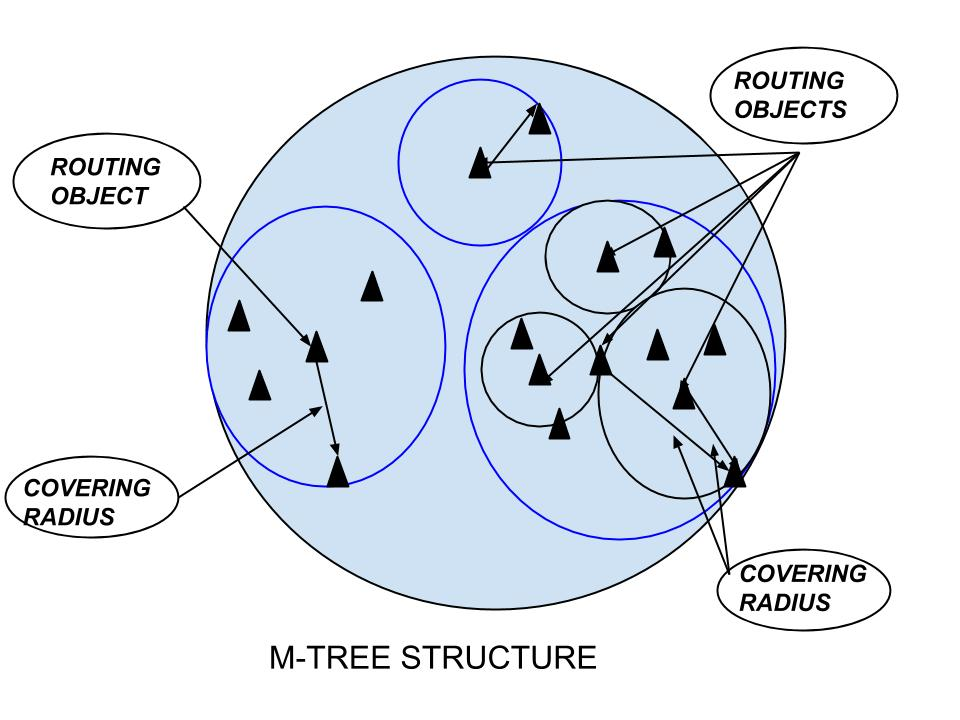
\includegraphics[width=0.55 \columnwidth]{img/mtree.jpg}
\caption{M-tree Structure Overview}
\end{figure}
	
\end{itemize}
\end{overlayarea}
\end{frame}

\begin{frame}
\frametitle{Indexing approach ...}
\begin{overlayarea}{\textwidth}{.8\textheight}
\begin{itemize}
	\item<1-> Select pivots? Number?
	\begin{itemize}
	\item<2-> The $i^{th}$ pivot is chosen such that its minimum distance to the previous $i-1$ pivots is maximized.
	\end{itemize}
	\item<3-> Assign each point to a pivot.
	\item<4->[]	
\begin{figure}[ht]	
\centering
\includegraphics<3->[width=0.5 \columnwidth]{img/image0a.jpg}
\end{figure}

\end{itemize}
\end{overlayarea}	
\end{frame}


\begin{frame}
\frametitle{Indexing approach ...}
\begin{overlayarea}{\textwidth}{.8\textheight}
\begin{itemize}
	\item<1-> Choose outliers ?	
	\item<2->[] 
\begin{figure}

\centering
\includegraphics<2->[width=0.5 \columnwidth]{img/image0b.jpg}
\end{figure}

\end{itemize}
\end{overlayarea}	
\end{frame}
	


\begin{frame}
\frametitle{Indexing approach}
\begin{overlayarea}{\textwidth}{.8\textheight}
  \begin{itemize}
	\item<1-> Repeat procedure on outlier set. 
	\item<2->[] 
\begin{figure}[ht]	
\centering
\includegraphics<2->[width=0.6 \columnwidth]{img/image0e.jpg}
\end{figure}
	\item<3-> Termination?	

\end{itemize}
\end{overlayarea}
	\end{frame}

\begin{frame}
\frametitle{Range Search}
\begin{itemize}
	\item Start from the root as pivot $p$
	\item Apply triangle inequality bounds to prune or include all  points from sub-tree.
	\item If not, then go to the children of $p$ and repeat the process with them as the new pivot, till we reach leaf.
	
%	\item Covering radius of pivot $p_i$ being $r_i$, the maximum distance of any node in $S_i$ (subtree rooted at $p_i$) to the query $q$ will be $dist(q,p_i)$ + $r_i$.
%	\item Use threshold $t$, to include the whole sub-tree.
\end{itemize}
\end{frame}

%\begin{frame}
%\frametitle{Range Search ...}
%\begin{itemize}
%	\item Similarly the minimum distance of any node in $S_i$ is $max(dist(q,p_i)$ - $r_i, 0)$. 
%	\item Prune?	
%	\item If not, then go to the children of $p_i$ and repeat the process till we reach leaf.
%\end{itemize}
%\end{frame}

\subsection{Inverted Index}
\begin{frame}
\frametitle{Inverted Index}
	\begin{itemize}
		\item High dimensionality and sparsity of chemical data are an impediment to our indexing process.
		\item Use of inverted index motivated by its use in text mining.
	\end{itemize}

\begin{figure}[ht]	
\centering
\includegraphics<1->[width=0.5 \columnwidth]{img/feature.jpg}
\caption{Distribution of data points against the features}
\end{figure}

\end{frame}

%\begin{frame}
%\frametitle{Indexing process}
%\begin{itemize}
%	\item Index on features.
%	\item Pre-processing?
%\end{itemize}
%\end{frame}

\begin{frame}
\frametitle{Range Search}
\begin{overlayarea}{\textwidth}{.8\textheight}
\begin{itemize}

\item<1->[]
\begin{figure}[ht]	
\centering
\includegraphics<1->[width=0.75 \columnwidth]{img/image0c.jpg}
\end{figure}

\end{itemize}
\end{overlayarea}	
\end{frame}


\begin{frame}
\frametitle{Pruning}
\begin{overlayarea}{\textwidth}{.8\textheight}
\begin{itemize}

\item<1->[]
\begin{figure}[ht]	
\centering
\includegraphics<1->[width=0.75 \columnwidth]{img/image0c1.jpg}
\end{figure}

\end{itemize}
\end{overlayarea}	
\end{frame}


%\begin{frame}
%\frametitle{Pruning features for binary fingerprints}
%\begin{itemize}
%	\item Consider $f_i$, if the following were to hold:  
%	\begin{equation}
%	\frac{1}{N_q - 1 + V_{i}}  < 1-t
%	\end{equation}
%	we can prune the feature $f_i$
%	
%	\item {Note: Here $t$ is the threshold distance, $V_{i}$ is the minimum number of features present among all points having the feature $f_i$}
%	
%		
%\end{itemize}
%\end{frame}

%\begin{frame}
%\frametitle{Proposed bounding theorem}
%\begin{theorem}
%\label{thm2bound}
%For a case of binary fingerprints, given a query $q$ and a threshold $t$, consider the feature set $F=f_1, f_2,...f_M$. If $P$ is the set of points from the database, which has atleast one of the features $f_k$  $(f_k~\in F)$ set to 1, then, we can prune all such points $p_j$ of P from being present in the candidate range search set for query compound $q$ if $p_j$ does not have any other common feature other than in the set $F$, and it follows the following bound. 
%
%\begin{equation}
%\label{eq:boun2}
%\frac{M}{N_q - 1 + \min\limits_{i\in~(1,M)}(V_i) } < 1-t 
%\end{equation}
%
%where $M$ is the number of features in the set $F$,\\ $N_q$ is the number of features in query q,\\$V_{i}$ is the minimum number of features present among all points having the feature $f_i$.
%
%\end{theorem}
%\end{frame}

\begin{frame}
\frametitle{Greedy Technique}

\begin{itemize}
	\item<1-> Sort the features based on popularity
	\item<2-> Hence if till the $i^{th}$ feature is considered, if j features (call it set $R$) have been pruned till now, we can prune the $i^{th}$ feature as well if the following holds.
	\begin{equation}
	\label{eq: greedy}
	\frac{j+1}{N_q - 1 + min(V_{i}, \rho)} < 1-t 
	\end{equation}
	
where 	$\rho$ is the minimum  number of features present in any point containing atleast one of the features pruned until now i.e $\rho = \min\limits_{k\in R} V_k$ 

\end{itemize}
\end{frame}

\begin{frame}
\frametitle{Extension to non-binary fingerprints}
%\begin{theorem}
Prune $i^{th}$ feature if:
\begin{equation}
\label{eq:boun3}
\frac{min(j_i,W_i)}{S_q - W_i -k_i+ l_i + max (k_i, V_i)}  < 1-t
\end{equation}
Here $j_i$ is the maximum feature value taken for the feature $f_i$,\\  $W_i$ is the $i^{th}$ feature value of query $q$,  \\$S_q$ is the sum magnitude of the feature values of the query $q$, \\ $k_i$ is the is the minimum feature value taken for the feature $f_i$,\\  $l_i$ is the minimum sum of feature values for any point containing the feature $f_i$ , \\ $t$ is the threshold similarity.
%\end{theorem}	
\end{frame}

\section{Experiments and Results}
\begin{frame}
\frametitle{Experiments}
\begin{itemize}
\item<1-> Datasets
\begin{itemize}
	\item PubChem Dataset (264016 compounds, 785985 features)
	\item DUD Dataset (128374 compounds, 32198 features)
\end{itemize}

\item<1-> Evaluations
\begin{itemize}
	\item Compare range search result with that of full database scan
	\item Compare average runtime of range search with the Bit bound technique 
\footnote{\textbf{Source:} Swamidass, S Joshua and Baldi, Pierre. \textit{Bounds and algorithms for fast exact searches of chemical fingerprints in linear and sublinear time.}} 
\end{itemize} 
\end{itemize}

\end{frame}

%\begin{frame}
%\frametitle{Statistics on data}
%\begin{table}[ht!]
%\centering
%\caption{Data Analysis: Statistics of the data-set PubChem-n}
%\begin{tabular}{|l|c|}
%\hline 
%Number of data points & 264016 \\ 
%Number of unique features is & 785985 \\ 
%Maximum number of features in a data point is & 1903 \\ 
%Minimum number of features in a data point is  & 7 \\ 
%Average number of features in a data point is & 270.602966 \\ 
%Maximum number of data points with a feature is & 259110 \\ 
%Minimum number of data points with a feature is & 1 \\ 
%Average number of data points with a feature is & 90
% \\ 
%Maximum value of a feature  & 1870 \\ 
%Minimum value of a feature
% & 1 \\ 
%Average value of a feature & 1.142210 \\ 
%Maximum number of heavy-hitters  & 144 \\ 
%Minimum number of heavy-hitters  & 1 \\ 
% Average number of heavy-hitters  & 44.5 \\ 
%\hline 
%\end{tabular} 
%\end{table}
%\end{frame}

\begin{frame}
\frametitle{M-tree based index analysis}
\begin{itemize}
	\item Indexing time per compound on average increases linearly with data-set size as well as with size of pivot-set
	\item Outlier base limit size has no significant effect. 
\end{itemize}
\end{frame}


\begin{frame}
\frametitle{M-tree based index analysis...}
\begin{overlayarea}{\textwidth}{.8\textheight}
\begin{itemize}

	\item<1-> Runtime for different pivot-set sizes? High v/s low?
	\item<2->[]
\begin{figure}[ht]	
\centering
\includegraphics<2->[width=0.75 \columnwidth]{img/image5.jpg}
\end{figure}

\end{itemize}
\end{overlayarea}
\end{frame}


\begin{frame}
\frametitle{Inverted index analysis}
\begin{itemize}
	\item<1-> Indexing time per compound on average is constant. Does not change with data-set size. 
	\item<2-> Pruning upto 50-100 features on average for low threshold distances. 
\end{itemize}
\end{frame}

\begin{frame}
\frametitle{Comparison}
\begin{figure}[ht]	
\centering
\includegraphics<1->[width=0.75 \columnwidth]{img/imageC1.jpg}
\caption{PubChem-n dataset}
\end{figure}
\end{frame}

\begin{frame}
\frametitle{Comparison ...}
\begin{figure}[ht]	
\centering
\includegraphics<1->[width=0.75 \columnwidth]{img/imageC2.jpg}
\caption{PubChem-b dataset}
\end{figure}
\end{frame}

\begin{frame}
\frametitle{Comparison ...}
\begin{figure}[ht]	
\centering
\includegraphics<1->[width=0.75 \columnwidth]{img/imageC3.jpg}
\caption{DUD dataset}
\end{figure}
\end{frame}

\section{Conclusion}
\begin{frame}
\frametitle{Conclusion}
\begin{itemize}
	\item<1-> Proposed an M-tree based index approach which achieved 2-3 times speed-up over the Bit-Bound Technique. 
	\item<2-> Proposed a novel inverted indexing technique which achieved 5-6 times speed-up over the Bit-Bound Technique.
	\item<3-> Showed the effectiveness of our techniques through comprehensive analysis on 2 real world datasets (both binary and non-binary).
\end{itemize}

\end{frame}

\begin{frame}
\begin{center}
	Thank You!
\end{center}
\end{frame}

\end{document} 
